\documentclass[a4paper,12pt]{article}

\usepackage[utf8]{inputenc}
\usepackage[polish]{babel}
\usepackage[OT4]{polski}

\usepackage[colorlinks=true,linkcolor=blue,urlcolor=blue]{hyperref}

\usepackage[pdftex]{graphicx}

%\linespread{1.2}


\title{Projekt z Metod Odkrywania Wiedzy\\Prezentacja uzyskanych wyników\\\Large{Proste algorytmy klasyfikacji tekstu. Porównania ze standardowymi algorytmami klasyfikacji dostępnymi~w~R.}\\}

\author{Marcin Chwedczuk, Piotr Monarski}
\date{}

\begin{document}
\maketitle

\section{Wstęp}

\section{Wstępne przetwarzanie surowych danych}
	\subsection{Opis danych}
		Jako dane uczące oraz testowe postanowiliśmy wykorzystać
		zbiór \textit{NSF Research Award Abstracts 1990-2003 Data Set}
		\cite{abstracts}
		wchodzący w skład repozytorium UCI.
		Zbiór ten zawiera 129 tysięcy streszczeń artykułów naukowych 
		w języku angielskim,
		które zostały nagrodzone przez National Science Foundation.
		Każdemu streszczeniu towarzyszy szereg informacji zawierających
		między innymi nazwiska autorów artykułu, tytuł artykułu oraz
		dziedzinę zastosowań (przy czym artykuł może mieć więcej 
		niż jedną dziedzinę zastosowań).
		Łączny rozmiar nieskompresowanego zbioru danych to ponad 400 MB.
		
		W naszej pracy wykorzystujemy jedynie część tego ogromnego zbioru 
		danych dystrybuowaną w postaci pliku \texttt{Part1.zip} i zawierającą
		zwycięskie artykuły naukowe z lat 1990 - 1994 (łącznie 10 097 streszczeń).
		\begin{figure}[htb]
			\centering
			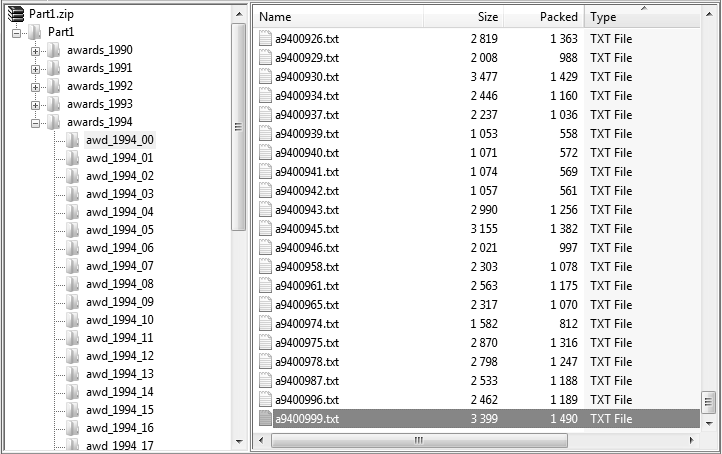
\includegraphics[scale=0.45]{./img/part1_dir_struct}
			\caption{Struktura katalogów zawartych w archiwum \texttt{Part1.zip}}
		\end{figure}
		
		Za opis pojedynczego artykułu naukowego odpowiada pojedynczy plik
		\texttt{.txt} o strukturze przedstawionej na rysunku
		\ref{fig:textstruct}. W ramach naszego projektu wykorzystujemy  
		jedynie pola \texttt{Fld Applictn} oraz \texttt{Abstract}, 
		zawierające odpowiednio dziedziny do których należy artykuł oraz
		jego streszczenie.
		\begin{figure}[!h]
			\scriptsize
			\begin{verbatim}
Title       : Large Scale Structure and Dynamics of Non-Equilibrium Systems
Type        : Award
NSF Org     : DMR 
Latest
Amendment
Date        : November 4,  1992   
File        : a9013984

Award Number: 9013984
Award Instr.: Continuing grant                             
Prgm Manager: G. Bruce Taggart                        
	      DMR  DIVISION OF MATERIALS RESEARCH          
	      MPS  DIRECT FOR MATHEMATICAL & PHYSICAL SCIEN
Start Date  : November 1,  1990   
Expires     : October 31,  1993    (Estimated)
Expected
Total Amt.  : $195000             (Estimated)
Investigator: Michael Cross mcc@caltech.edu  (Principal Investigator current)
Sponsor     : California Inst of Tech
	      1201 E California Blvd
	      Pasadena, CA  911250001    818/795-4571

NSF Program : 1765      MATERIALS THEORY
Fld Applictn: 0106000   Materials Research                      
              13        Physics                                 
Program Ref : 9161,
Abstract    :
                                                                                             
              The PI proposes a theoretical study of the large scale and slow                
              dynamics of spatially extended non-equilibrium systems.  Two                   
              classes of model systems will be investigated: 1. one and two                  
              dimensional lattices of discrete chaotic elements or oscillators               
              with dynamics preserving a conserved quantity or having an internal            
              symmetry; 2. two dimensional fluid flow.  Numerical simulation,                
              Monte Carlo methods, mean field theory, and renormalization group              
              methods will be used.
			\end{verbatim}
			\caption{Przykładowy plik opisujący artykuł naukowy}
			\label{fig:textstruct}		
		\end{figure}
	
	\subsection{Etap I: Usuwanie nieznaczących informacji}
		Pierwszy etap przetwarzania danych ma na celu usunięcie z powyżej
		opisanych plików \texttt{.txt} informacji nieistotnych z naszego punktu
		widzenia. Po przetworzeniu każdy plik \texttt{.txt} będzie miał 	
		następującą strukturę:
		\begin{verbatim}
dziedzina_1, dziedzina_2, ..., dziedzina_N
(pusta linia)
Treść streszczenia artykułu naukowego w pojedynczej linii
		\end{verbatim}
		Dokładniej plik będzie składał się z trzech linii:
		\begin{itemize}
			\item
				Pierwszej zawierającej nazwy dziedzin zastosowań danego artykułu
				oddzielone znakiem przecinka (wymagana jest obecność co najmniej
				jednej dziedziny)
			\item
				Drugiej która pełni rolę separatora i nie zawiera żadnych 
				danych
			\item
				Trzeciej która zawiera streszczenie artykułu ze znakami 
				\verb+\n+ i \verb+\r+ zamienionymi na spacje
				(ta linia musi zawierać co najmniej 30 znaków)
		\end{itemize}
				
		Dodatkowym rezultatem etapu I będzie usunięcie ze zbioru danych 
		opisów artykułów które nie zawierają dziedzin(-ny) zastosowań lub
		posiadają zbyt krótkie streszczenia.
		
		Wstępne przetwarzanie danych należy wykonać w 
		następujący sposób:
		\begin{enumerate}
			\item
				Najpierw kopiujemy wszystkie pliki \verb+.txt+ zawarte
				w archiwum \texttt{Part1.zip} do wybranego katalogu
				np. \verb+c:\data_in+. Skopiować należy wyłącznie pliki
				bez struktury katalogów
			\item
				Tworzymy katalog w którym znajdą się przetworzone pliki
				np. \verb+c:\data_out+. Następnie korzystamy z
				funkcji \texttt{preprocess} zawartej w naszym pakiecie języka R:
				\begin{verbatim}
preprocess('c:\data_in', 'c:\data_out');
				\end{verbatim}
				Po zakończeniu działania funkcji \texttt{preprocess} katalog
				\verb+c:\data_out+ powinien zawierać przetworzone pliki
				\verb+.txt+ o nazwach zgodnych z ich oryginalnymi odpowiednikami
		\end{enumerate}	
		
		\textsc{UWAGA:} Aby zaoszczędzić użytkownikom czasu niezbędnego
		do wykonania powyższych kroków przygotowaliśmy skrypt 
		\verb+data_preprocessing_report.R+ który wykonuje opisane wyżej
		czynności. Aby skorzystać ze skryptu należy zmodyfikować
		linie:
		\begin{verbatim}
# Sciezka do katalogu ktory zawiera rozpakowane
# archiwum Part1.zip
org.data.directory <- 'D:/tmp/words/Part1/'

# Sciezka do katalogu ktory bedzie zawieral
# przetworzone dane oraz dane tymczsowe
data.directory <- 'd:/mtmp/';
		\end{verbatim}
		Po wykonaniu skryptu katalog wskazany jako \verb+data.directory+
		powinien zawierać podkatalog \verb+data_preprocessed+ zawierający
		wstępnie przetworzone pliki artykułów (około 47 tysięcy plików).	
	
	\subsection{Etap II: Konwersja na ramkę danych}
		Drugi etap przetwarzania danych polega na zamianie zbioru
		plików utworzonych na etapie I na ramkę danych.
		
		Utworzona ramka danych będzie miała format przedstawiony w
		tabeli \ref{t:df}.
		\begin{table}[!h]	
			\begin{center}	
			\small			
			\begin{tabular}{|c|c|c|c|c|c|c|c|}
				\hline
				w.word1 & w.word2 & \ldots & w.wordN & c.class1 & \ldots & c.classM & Informacje dodatkowe \\
				\hline \hline
				5 & 5 & \ldots & 57 & 2 & \ldots & 2 & (nie dotyczy) \\
				\hline
				1 & 0 & \ldots & 3 & 0 & \ldots & 1 & art1.txt \\
				\hline
				0 & 2 & \ldots & 0 & 1 & \ldots & 0 & art2.txt \\
				\hline
				4 & 3 & \ldots & 54 & 1 & \ldots & 1 & art3.txt \\
				\hline
			\end{tabular}	
			\end{center}				
		
			\caption{Format ramki danych utworzonej w wyniki II etapu
			przetwarzania danych dla trzech plików art1.txt, art2.txt oraz
			art3.txt}
			\label{t:df}
		\end{table}
		Każdemu plikowi \texttt{.txt} zawierającemu streszczenie i 
		dziedziny zastosowań będzie odpowiadał pojedynczy wiersz ramki danych.
		Dodatkowo pierwszy wiersz tabeli nie odpowiada żadnemu plikowi
		\texttt{.txt}, ale zawiera pomocnicze dane statystyczne.
		Dokładniej dla danej kolumny zawierającej wartości numeryczne,
		pierwszy wiersz zawiera sumę elementów pozostałych wierszy w
		kolumnie.
		
		W przypadku kolumn zastosowano następujące kodowanie, kolumna 
		której nazwa ma format \texttt{w.xxyyzz}, odpowiada słowu
		\texttt{xxyyzz}. Dla wiersza opisującego streszczenie artykułu
		kolumna \texttt{w.xxyyzz} zawiera \emph{ilość wystąpień}
		słowa \texttt{xxyyzz} w streszczeniu.
		
		Kolumny o nazwach postaci \texttt{c.xxyyzz} a więc rozpoczynających
		się od ,,c.'' niosą informacje o dziedzinach zastosowań artykułu.
		Każda z tych kolumn może zawierać jedynie wartości 1 lub 0, mówiące
		o tym czy dany artykuł należy do danej klasy (dziedziny zastosowań).
		
		W ramce występują również kolumny o nazwach rozpoczynających się od
		,,meta.'' które niosą informacje dodatkowe takie jak np. nazwa pliku
		na podstawie którego wygenerowany został dany wiersz tablicy.
		
		Zamiana zbioru plików \texttt{.txt} utworzonych w ramach I etapu
		będzie przebiegała następująco:
		\begin{enumerate}
			\item
				Zamian wszystkich znaków występujących w streszczeniach
				i nie będących literami na spacje
			\item
				Zamiana dużych liter na małe litery, usuwanie wielokrotnych
				powtórzeń białych znaków, usuwanie białych znaków z początku
				i końca tekstu streszczenia
			\item
				Stemming tekstów za pomocą funkcji \texttt{wordStem}
				z pakietu \texttt{Rstem}
			\item
				Usuwanie \textit{stopwords} (wykorzystano listę
				angielskich stopwords opublikowaną w internecie,
				szczegóły znajdują się w pomocy do funkcji \texttt{is.stop.word}
				)
			\item
				Na podstawie tak uzyskanej listy słów alokacja kolumn
				ramki danych
			\item
				Ustalenie występujących w artykułach dziedzin zastosowań
			\item
				Tworzenie ramki danych. Dla danego wiersza odpowiadającego
				streszczeniu X, kolumna typu w.abc odpowiada liczbie wystąpień
				słowa abc w przetworzonym tekście X, a kolumna c.abc zawiera 
				1 gdy abc jest dziedziną zastosowań artykułu 
				którego streszczeniem jest X
		\end{enumerate}
		
		Za wykonanie opisanych wyżej przekształceń odpowiada 
		funkcja 
		\begin{verbatim}
create.aritcles.data.frame(articles.directory, output.df.filename)
		\end{verbatim}
		przyjmująca jako parametry ścieżkę do katalogu zawierającego
		wstępnie przetworzone pliki \texttt{.txt}, oraz ścieżkę do 
		pliku w którym ma zostać zapisana ramka danych.
		
		Ponieważ utworzony plik ramki danych może być znacznych rozmiarów
		(powyżej 500MB), zalecamy wczytanie ramki danych oraz ponowny 
		jej zapis w postaci binarnej za pomocą funkcji \texttt{save}.
		Pozwoli nam to zaoszczędzić czasu związanego z parsowaniem
		pliku ASCII (utworzony plik ramki ma format tekstowy).
		\begin{verbatim}
df <- read.table('articles.df', header=TRUE);
save(df, file='articles.bin', compress=FALSE);
		\end{verbatim}		
				
		\textsc{UWAGA}: Jeżeli możemy poświęcić dodatkowo 1GB przestrzeni
		dyskowej to lepiej dokonać zapisu bez kompresji - spowoduje to
		zmniejszenie obciążenia pamięci podczas wczytywania ramki oraz
		skrócenie czasu wczytywania danych.
	
\section{Wektoryzacja danych}
		Utworzona w poprzednim punkcie tego dokumentu ramka danych
		zawiera około XXX tysięcy wierszy oraz YYY tysięcy kolumn.
		Niestety taki rozmiar danych okazał się zbyt dużym obciążeniem
		dla wykorzystywanych przez nas algorytmów. Dodatkowo okazało się
		że większość algorytmów oczekuje pojedynczych etykiet dla danych
		ze zbioru trenującego. Z tych względów zdecydowaliśmy się 
		na dodatkowe przetworzenie zbioru danych które pozwoli na jego
		kompresję oraz rozwiąże problem wielokrotnych kategorii.
		
		Najpierw zajmiemy się problemem zbyt dużego rozmiaru danych:
		\begin{enumerate}
			\item
				Usuwamy te kolumny kategorii które są reprezentowane
				przez mniej niż \texttt{min.n} streszczeń
			\item
				Usuwamy kategorie ogólne np. c.OtherApplicationsNEC lub
				c.OtherSciencesNEC
			\item
				Usuwamy wiersze które nie należą do żadnej z kategorii
				(takie wiersze mogły się pojawić po wykonaniu kroków 1 i 2)
			\item
				Usuwamy kolumny odpowiadające słowom które występują
				w mniej niż \texttt{min.n} razy
			\item
				Usuwamy informacje dodatkowe (kolumny rozpoczynające się
				od ,,meta.'')
		\end{enumerate}
		
		Teraz rozwiążemy problem wielokrotnych kategorii:
		\begin{enumerate}
			\item
				Każdy wiersz który należy do klas $c_1$, $c_2$, \ldots, $c_N$
				zamieniamy na $N$ wierszy danych takich że pierwszy należy
				do kategorii $c_1$, drugi do kategorii $c_2$ itd.
		\end{enumerate}
		
		Za przeprowadzenie wyżej opisanych operacji jest
		odpowiedzialna funkcja \texttt{vectorize.data}:
		\begin{verbatim}
lst <- vectorize.data(
    df, min.n, 
    create.hash(c("c.OtherApplicationsNEC", "c.OtherSciencesNEC")),
    min.w);
		\end{verbatim}
		
		Parametry funkcji \texttt{vectorize.data}: \texttt{min.w} oraz
		\texttt{min.n} zostaną dołączone do parametrów algorytmów
		które uczą się na zwektoryzowanych danych.

\section{Zastosowane algorytmy}
	\subsection{Algorytm kNN}
	\subsection{Algorytm Naive Bayes}
	
	\subsection{Algorytm Multinomial Bayes}	
		\textsc{DANE WEJŚCIOWE}: Zwektoryzowana ramka danych zawierająca
		liczby wystąpień poszczególnych słów\\
		\textsc{DANE WYJŚCIOWE}: Model danych do wykorzystania w funkcji
		\texttt{predict}\\	
		
		Oba zaprezentowane tutaj algorytmy pochodzą z
		13 rozdziału pozycji \cite{irbook}.
	
		\subsubsection{Wersja I}
		\begin{figure}[!h]
			\centering
			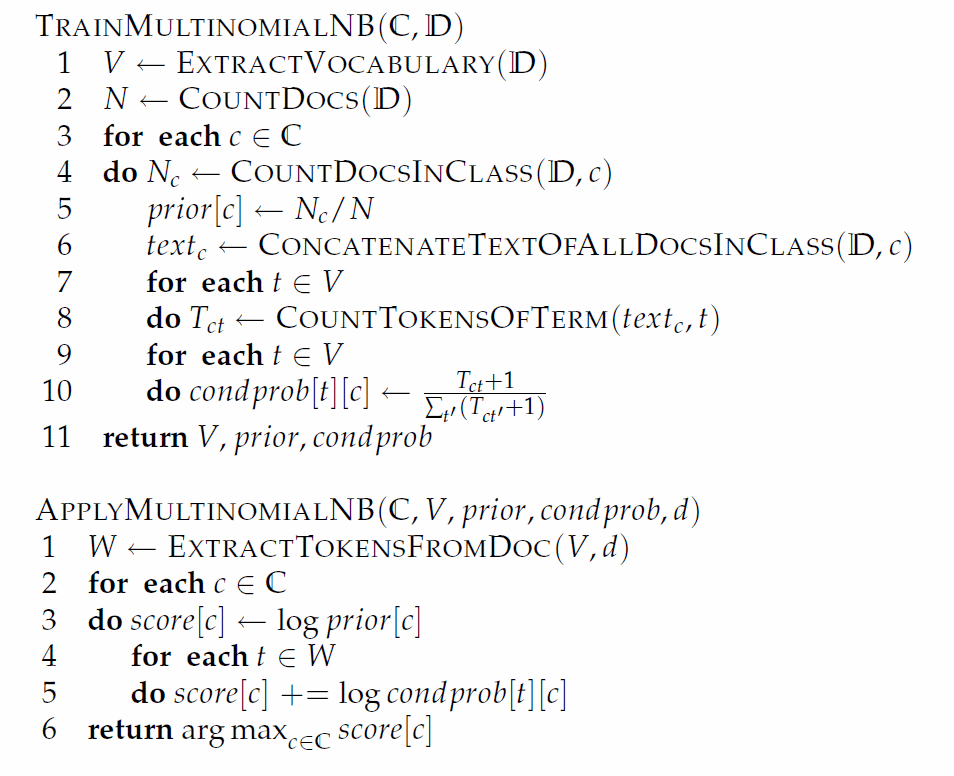
\includegraphics[scale=0.45]{./img/mnbalg}
			\caption{Pseudokod algorytmu Multinomial Naive Bayes}
		\end{figure}
		
		\subsubsection{Wersja II}
		\begin{figure}[!h]
			\centering
			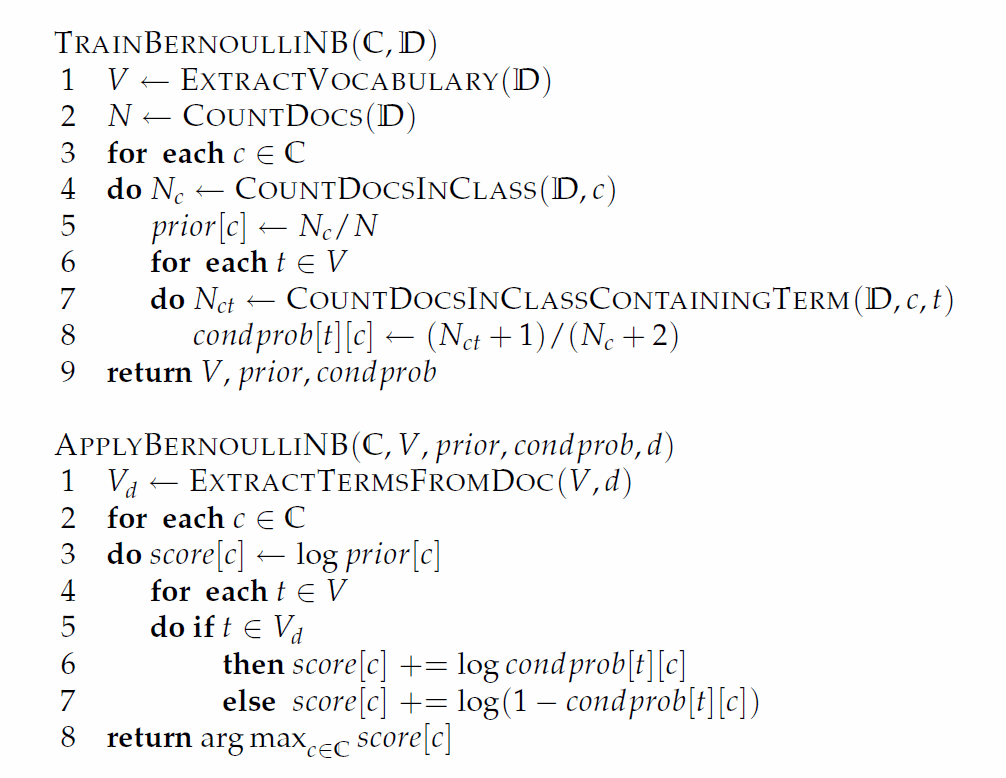
\includegraphics[scale=0.45]{./img/bnbalg}
			\caption{Pseudokod algorytmu Bernoulli Naive Bayes}
		\end{figure}		

		\subsubsection{Przykład użycia}
		Poniżej przedstawiamy przykład użycia poszczególnych algorytmów.
		W poniższych listingach będziemy zakładać że zmienna \texttt{lst}
		została zwrócona przez funkcje \texttt{vectorize.data}.
		\begin{verbatim}
test <- sample(1:nrow(lst$data), 900, replace=FALSE)

test.data <- lst$data[test,]
test.cls  <- lst$fact[test,]
row.names(test.data) <- NULL

learn.data <- lst$data[-test,]
learn.cls  <- lst$fact[-test,]
row.names(learn.data) <- NULL

model <- train.multinomial.nb(data=learn.data, fact=learn.cls)
# lub
model <- train.bernoulli.nb(data=learn.data, fact=learn.cls)

# algorytmy zwracaja tablice p-stwa
# przenaleznosci przykladu do poszczegolnych
# klas
p <- predict(model, test.data);
c <- apply(p, 1, function(r) which(r == max(r)))
table(p, test.cls)
		\end{verbatim}
		
		\clearpage
	
\section{Wykorzystywane algorytmy pakietu R}

	\subsection{Funkcja \texttt{naiveBayes} z pakietu \texttt{e1071}}
	
	Sygnatura funkcji \texttt{naiveBayes} wygląda następująco:
\begin{verbatim}
naiveBayes(formula, data, laplace = 0, ..., subset, na.action = na.pass)
\end{verbatim}
	Funkcja była wywoływana na dokładnie tych samych danych co
	pozostałe algorytmy. 
	
	Poniżej przedstawiamy przykładowe 
	wywołanie funkcji przy założeniu że zmienna \texttt{lst}
	została zwrócona przez funkcje \texttt{vectorize.data}.
\begin{verbatim}
data <- lst$data;
tmp  <- colnames(lst$data);
data.class <- lst$fact;

formula.string <- paste(tmp, collapse=' + ');
formula.string <- paste('class ~', formula.string);
f <- formula(formula.string);

model <- naiveBayes(f, data, laplace);
\end{verbatim}
	
	\subsection{Funkcja \texttt{rpart} z pakietu \texttt{rpart}}
	
	Funkcja \texttt{rpart} buduje modele klasyfikacji w oparciu 
	o drzewa decyzyjne, sygnatura funkcji wygląda następująco:
\begin{verbatim}
rpart(formula, data, weights, subset, na.action = na.rpart, method,
      model = FALSE, x = FALSE, y = TRUE, parms, control, cost, ...)
\end{verbatim}
	
	Funkcja była wywoływana w następujący sposób:
\begin{verbatim}
data <- lst$data;
tmp  <- colnames(lst$data);
data.class <- lst$fact;

formula.string <- paste(tmp, collapse=' + ');
formula.string <- paste('class ~', formula.string);
f <- formula(formula.string);

model <- rpart(f, data, method="class");
\end{verbatim}

\section{Uzyskane wyniki}

\section{Wnioski}

% --------------------------------------------
% BIBLIOGRAFIA
% --------------------------------------------

\begin{thebibliography}{9}

\bibitem{abstracts}
   \emph{NSF Research Award Abstracts 1990-2003 Data Set}.
   \url{http://archive.ics.uci.edu/ml/datasets/NSF+Research+Award+Abstracts+1990-2003}
\bibitem{irbook}
	\emph{An Introduction to Information Retrieval}. 
	C. D. Manning, P. Raghavan, H. Sch\"utze.
	Cambridge University Press.
	Wersja online: \url{http://nlp.stanford.edu/IR-book/html/htmledition/irbook.html}
\bibitem{wikistemming}
	Wikipedia, Stemming, \url{http://en.wikipedia.org/wiki/Stemming}

\end{thebibliography}


\end{document}
